\section{Views or pixels: spending a token budget}
\label{sec:budget}

So far the mix was given. Now suppose the budget can be spent freely. Should one mix resolutions, or use uniform views?

\paragraph{Design.}
For each model and budget, we choose on the selection seed the best uniform input U from a grid of 2 to 32 views, and the best mix X from the mixed inputs of our selection studies. Both choices were frozen before any reporting-seed job ran.

\paragraph{Pose: uniform input wins.}
U beats X in 10 of 24 pose cells, X beats U in 1, and 13 are inconclusive. If mixing paid off where tokens are scarcest, its advantage would grow as the budget shrinks. We predicted this and ran the 4{,}096-token choices at 2{,}048 tokens; the prediction failed. At 2{,}048 tokens, U wins 7 of 15 cells and X none, and on HiRoom \pithree loses 21.6 \auc with the mix.

\paragraph{Reconstruction: the mix seems to help, but because of its views.}
For reconstruction the picture is less clear. X wins 3 cells, loses 3, and leaves 18 inconclusive. On held-out DTU at 4{,}096 tokens, X lowers the Chamfer distance for \pithree from 7.28\,mm to 5.64\,mm and for \dathree from 6.64\,mm to 5.11\,mm; all cells at 8{,}192 tokens are inconclusive. These wins come with a confound. The best mixes use 10 to 12 views, while the best uniform inputs usually use 8. The uniform grid simply had no 10- or 12-view option, so U and X differ in view count as well as in how resolution is spread.

We therefore added uniform inputs with 10 and 12 views at the same budgets (U10, U12) and predicted that they would match or beat the mix, which is what we found. On DTU at 4{,}096 tokens, 12 uniform views reach 5.56\,mm for \pithree, against 5.64\,mm for the mix, and 4.44\,mm for \dathree, against 5.11\,mm. Over all reconstruction comparisons, the mix wins 4 and loses 6 of 30 against U10, and wins 2 and loses 5 of 24 against U12: 6 wins and 11 losses in 54 (\cref{fig:budget}). \Cref{tab:eth3d} shows the clearest case. On ETH3D, \pithree's mix beats the best uniform input from the grid at both budgets, yet 12 uniform views beat the mix by 0.208 in F-score at 8{,}192 tokens. The same holds when the mix's own frames are used: putting all of X's frames at one size, at equal tokens, matches or beats the mix for \pithree (ETH3D at 4{,}096 tokens: the mix is $+0.050$ ahead, not significant; ETH3D at 8{,}192 and HiRoom at 4{,}096: the mix is behind by 0.027 and 0.074, both significant).

\begin{figure}[t]
  \centering
  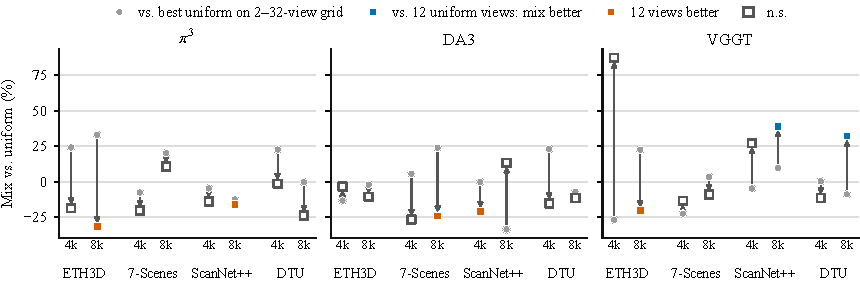
\includegraphics[width=\linewidth]{figures/fig_budget.pdf}
  \caption{\textbf{The mix's reconstruction gain is mostly a gain from extra views.} Relative difference of each model's frozen best mix X against its frozen best uniform input U from the 2--32-view grid (grey circles) and against 12 uniform views U12 (squares; filled when significant, blue = mix better, orange = 12 views better). F-score on ETH3D, 7-Scenes and ScanNet++; negated Chamfer distance on DTU. HiRoom is omitted because 11 of its 30 scenes have fewer than 12 frames. ETH3D uses 9 of 11 scenes.}
  \label{fig:budget}
\end{figure}

\begin{table}[t]
\centering\small
\setlength{\tabcolsep}{5pt}
\begin{tabular}{@{}lcccc@{}}
\toprule
Budget & U (grid best) & X (mix) & U10 & U12 \\
\midrule
4{,}096 & 0.374 & 0.464 & 0.404 & 0.571 \\
8{,}192 & 0.336 & 0.447 & 0.429 & \textbf{0.656} \\
\bottomrule
\end{tabular}
\caption{\textbf{Where mixing seems to pay, more views pay more.} \pithree reconstruction F-score on ETH3D (9 of 11 scenes). The mix X beats the best uniform input from the grid, but not 12 uniform views.}
\label{tab:eth3d}
\end{table}

\paragraph{One exception, and a caution.}
We found one setting where the mix beats every uniform input: VGGT on ScanNet++ at 8{,}192 tokens, with an F-score of 0.364 against 0.332 for U, 0.281 for U10 and 0.262 for U12. Since VGGT needs many tokens per view (\cref{sec:vggt}), the mix may help here by keeping a few views above that threshold. The caution is that pose and reconstruction prefer different inputs: compared with U, the 10- and 12-view inputs give worse pose in 23 of 54 comparisons and better pose in 4. DTU is the exception, where more views also help pose; for \dathree at 4{,}096 tokens, U scores 33.3 \auc and U10 scores 56.1.

\paragraph{Answer.}
When tokens can be allocated freely, the gain people expect from mixing resolutions is, in our results, mostly a gain from using more views. A uniform input with the right number of views is the better default for these models. The right number depends on the task: fewer, larger views for pose, more views for reconstruction.
